\documentclass[tikz, border=2pt]{standalone}
\usepackage{graphicx} 
\usepackage{tikz} 
\usepackage{tikz-3dplot} 
\usetikzlibrary{angles,quotes,arrows.meta, positioning} 
\usepackage{pgfplots} 
\pgfplotsset{compat=1.18} % Pacchetti Matematici 
\usepackage{amsmath, amssymb, amsthm} 

\definecolor{myblue}{HTML}{139FE9}
\begin{document}
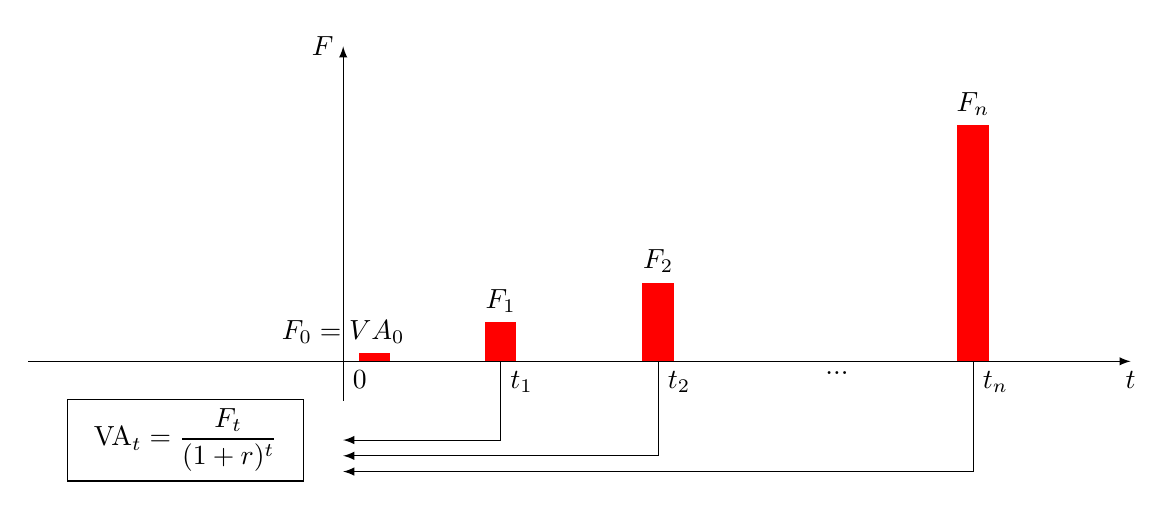
\begin{tikzpicture}[scale = 1]
        \tikzstyle{box} = [rectangle, draw,minimum width=3cm, minimum height=1cm, text centered]
        % Draw t-axis
        \draw[-latex] (-4,0) -- (10,0) node[below] {$t$};
        % Draw vertical lines
        \draw[-latex] (0,-0.5) -- (0,4) node[left] {$F$};
        % Draw lines for time points
        \draw(2,0) -- (2,-1) node[left]{};
        \draw(4,0) -- (4,-1.2) node[left]{};
        \draw(8,0) -- (8,-1.4) node[left]{};
        % Draw arrows for cash flows
        \draw[-latex](2,-1) -- (0,-1) node[left]{};
        \draw[-latex](4,-1.2) -- (0,-1.2) node[left]{};
        \draw[-latex](8,-1.4) -- (0,-1.4) node[left]{};
        % Label time points
        \node[below right] at (0,0) {$0$};
        \node[below right] at (2,0) {$t_1$};
        \node[below right] at (4,0) {$t_2$};
        \node[below right] at (6,0) {$...$};
        \node[below right] at (8,0) {$t_n$};
        % Optionally, label the height of the bars if known
        \node[above] at (0,0.1) {$F_0=VA_0$};
        \node[above] at (2,0.5) {$F_1$};
        \node[above] at (4,1) {$F_2$};
        \node[above] at (8,3) {$F_n$};
        % Add rectangles for future cash flows
        \fill[red] (0.2,0) rectangle ++(0.4,0.1);   % Width of 0.4, height based on F1
        \fill[red] (2-0.2,0) rectangle ++(0.4,0.5);   % Width of 0.4, height based on F1
        \fill[red] (4-0.2,0) rectangle ++(0.4,1);     % Width of 0.4, height based on F2
        \fill[red] (8-0.2,0) rectangle ++(0.4,3);     % Width of 0.4, height based on Fn
        % NPV formula box
        \node (VA) [box] at (-2,-1) {$\text{VA}_t = \displaystyle \frac{F_t}{(1+r)^t} $};
    \end{tikzpicture}
\end{document}